\documentclass[oneside]{article}

% ---------------------------------------------
% Importing packages
% ---------------------------------------------

% Encoding and font
\usepackage[utf8]{inputenc}
\usepackage{tgcursor}
\usepackage{hyperref}

% Different colors
\usepackage{xcolor}
\usepackage{color}
\definecolor{bluepoli}{cmyk}{0.4,0.1,0,0.4}

% Math
\usepackage{amsmath}
\usepackage{amsthm}

% Images
\usepackage{graphicx}
% \graphicspath{ {./Figures/} }

% Margins
\usepackage[a4paper, top=2cm, left=2.5cm, right=2.5cm, bottom=2cm]{geometry}

% Fancy header and footer
\usepackage{fancyhdr}
\pagestyle{fancy}
\fancyhf{}
\rhead{Calcoli di Processo dell'Ingegneria Chimica}
\lhead{Practical Session 5}
\rfoot{Page \thepage}
\lfoot{Academic Year 2024-2025}


\usepackage{amsthm}
\usepackage{tcolorbox}
\tcbuselibrary{most}
\tcolorboxenvironment{proof}{% `proof' from `amsthm'
   blanker,
   breakable,
   left=5mm,
   before skip=10pt,
   after skip=10pt,
   borderline west={1mm}{0pt}{bluepoli}
}

% ---------------------------------------------
% Title
% ---------------------------------------------

\title{Practical Session 5}
\author{Timoteo Dinelli\footnote{timoteo.dinelli@polimi.it}, Marco Mehl\footnote{marco.mehl@polimi.it}}
\date{8\textsuperscript{th} of November 2024}

% ---------------------------------------------
% Begin of the document
% ---------------------------------------------

\begin{document}
\maketitle

\section{``Boeing 737''}
Un Boeing 737 tocca la pista d'atterraggio ad una velocità $v = 210 \frac{km}{h}$.
Vengono subito attivati gli inversori di spinta per deviare i gas di scarico dell'aereo
nella stessa direzione del moto, ottenendo di conseguenza un'azione frenante. Si chiede
di calcolare la velocità d'uscita dei gas di scarico (relativa) che permette all'aereo di
fermarsi in un tempo $t = 15 \: s$.

\subsection*{Dati:}
\begin{itemize}
   \item massa iniziale BOEING = 35000 $kg$
   \item f = 0.97
   \item Sezione d'uscita gas di scarico = 0.085 $m^{2}$
   \item Area frontale investita dall'aria = 25 $m^{2}$
\end{itemize}

\subsection*{Soluzione:}
\begin{align}
   \frac{d(mv)}{dt} &= -2\dot{m}_{out} v_{out} - \frac{1}{2} f \rho v^{2} A \\
   m\frac{dv}{dt} &= -2\dot{m}_{out} (v_{out} - v) - \frac{1}{2} f \rho v^{2} A \\
   m\frac{dv}{dt} &= -2 \dot{m}_{out} v_{r} - \frac{1}{2} f \rho v^{2} A \\
   m(t) &= m_{0} - 2\dot{m} t \\
   (m_{0} - 2\dot{m}_{out} t )\frac{dv}{dt} &= -2\dot{m}_{out} v_{r} - \frac{1}{2} f \rho
   v^{2} A
\end{align}
\begin{align}
   \int_{v_{0}}^{0}\frac{dv}{2\dot{m}_{out} v_{r} + \frac{1}{2} f v^{2} A} &=-
   \int_{0}^{t} \frac{dt}{m_{0} - 2\dot{m}_{out} t} \\
   \dot{m}_{out} &= \rho S v_{r} \\
   \int_{v_{0}}^{0}\frac{dv}{2 S v_{r}^{2} + \frac{1}{2} f v^{2} A} &=-\rho \int_{0}^{t}
   \frac{dt}{m_{0} - 2\rho S v_{r} t}
\end{align}
\begin{equation*}
   \alpha = 2 S v_{r}^{2}, \quad \beta = \frac{1}{2} f A, \quad \gamma = m_{0}, \quad
   \delta = 2 \rho S v_{r}.
\end{equation*}

\begin{align}
   \int_{v_{0}}^{0} \frac{dv}{\alpha + \beta v^{2}} &= -\rho \int_{0}^{t}
   \frac{dt}{\gamma - \delta t} \\
   \int \frac{1}{\alpha + \beta x^{2}} dx &=
   \frac{atan\left(\sqrt{x\frac{\beta}{\alpha}}\right)}{\sqrt{\alpha \beta}} + c \\
   \int \frac{1}{\gamma - \delta x} dx &= -\frac{log\left(\gamma - \delta
   x\right)}{\delta} + c
\end{align}
\begin{equation}
   \label{eq:final}
   \frac{1}{\sqrt{\alpha\beta}} atan\left( v_{0} \sqrt{\frac{\beta}{\alpha}}\right) +
   \frac{\rho}{\delta}ln\left(1-\frac{\delta}{\gamma}t\right) = 0
\end{equation}

Rearrange equation number \ref{eq:final} as to be $\delta = ...$, after some simple steps
we obtain:

\begin{equation}
   \delta = \frac{\gamma}{t}\left(1-exp\left(-\frac{\delta}{\rho \sqrt{\alpha \beta}}
   atan\left(v_{0}\sqrt{\frac{\beta}{\alpha}}\right)\right)\right)
\end{equation}
\begin{equation*}
   \delta = 2 \rho S v
\end{equation*}
\begin{equation}
   v = \frac{\gamma}{2 \rho S t}\left(1-exp\left(-\frac{\delta}{\rho \sqrt{\alpha \beta}}
      atan\left(v_{0}\sqrt{\frac{\beta}{\alpha}}\right)\right)\right)
\end{equation}

\section{``Due serbatoi di Nafta (Esercitazione 5, Esercizio 9, MdF)''}
\begin{figure}[htp]
    \centering
    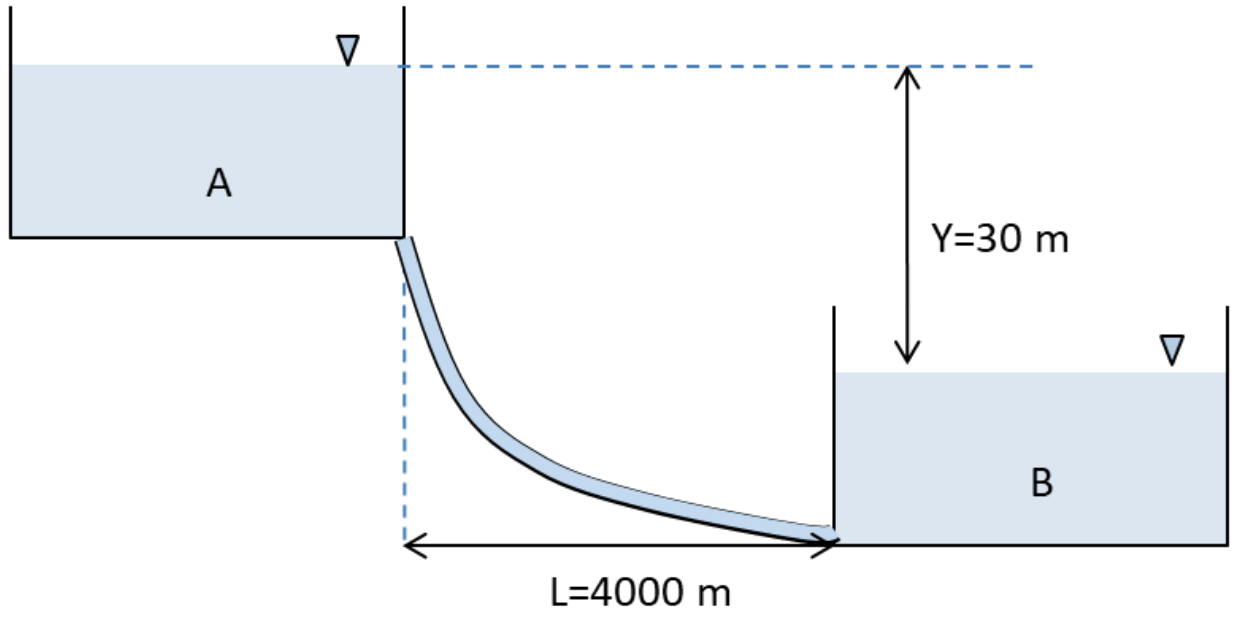
\includegraphics[width=.8\textwidth]{Serbatoi.png}
    \caption{Schematizzazione del sistema di collegamento di due serbatoi.}
    \label{fig:figura_2}
\end{figure}
Due serbatoi di nafta ($\mu = 0.039\:Pa\:s \quad \gamma = 8335 \:m^{3}$) le cui superfici
libere hanno un dislivello $Y$, sono collegati da una condotta di acciaio di lunghezza
$L = 4000 \: m$. Supponendo che la condotta abbia diametro costante pari a $D = 0.25 \: m$, si
determini la portata $\dot{V}$. Supponendo poi che occorra trasferire una portata
$\dot{V}^{'} = 1 \: \frac{m^{3}}{s}$, si determini il diametro teorico $D_{t}$ e si
dimensioni la condotta (coefficiente di scabrezza di Kutter $m = 0.5 \: m^{0.5}$). Il
sistema è schematizzato in Figura \ref{fig:figura_2}.

\subsection*{Soluzione}
Le perdite di carico distribuite sono calcolate tramite la relazione di Chèzy:
\begin{align}
   \Delta H &= \frac{v^2}{C^2 R_h}L \\
   C &= \frac{100 \sqrt{R_h}}{m + \sqrt{R_h}}
\end{align}
Il teorema di Bernoulli applicato tra i peli liberi dei due serbatoi fornisce:
\begin{equation}
   \label{eq:bern}
   Y = \Delta H = \frac{v^2}{\left(\frac{100\sqrt{D/4}}{m + \sqrt{D/4}}\right)D/4}L
\end{equation}
Per $D = 0.25 \: m$ si ha $\dot{V} = 0.0354 \: \frac{m^3}{s}$.\\
Considerando invece una portata pari a $\dot{V}' = 1 \: \frac{m^3}{s}$ e inserendo i
valori numerici nell' equazione \ref{eq:bern} si ottiene:
\begin{equation}
   \label{eq:tryerror}
   Y = \frac{10.37 \left(\sqrt{D/4} + 0.5\right)^2}{D^6}
\end{equation}
L'equazione \ref{eq:tryerror} si può risolvere tramite sostituzione successive. Ad
esempio, isolando il denominatore:

\begin{equation}
   D = \sqrt[6]{\frac{10.37 \left(\sqrt{D/4} + 0.5\right)^2}{Y}}
\end{equation}
\begin{equation}
   \label{eq:tobesol}
   D = 0.837 \sqrt[3]{\sqrt{D/4} + 0.5}
\end{equation}

L'equazione \ref{eq:tobesol} può essere vista come l'uguaglianza tra due funzioni: $y_1 =
D$ e $y_2 = 0.837\sqrt[3]{\sqrt{D/4} + 0.5}$ ed essere risolta in maniera efficiente per
sostituzioni successive. In realtà a partire dall' equazione \ref{eq:tryerror} si può
derivare la seguente equazione isolando il diametro $D$ a partire da
$\sqrt{\frac{D}{4}}$:

\begin{equation}
   D = 4 \left(\sqrt{\frac{Y D^6}{10.37}}- 0.5\right)^2
\end{equation}
E' facile dimostrare, graficamente, che questa scelta ci porta ad avere problemi di
convergenza in quanto si rischia di oscillare tra due soluzioni, matematicamente valide
ma fisicamente no.

\section{``Rubinetti in Serie''}
\begin{figure}[htp]
    \centering
    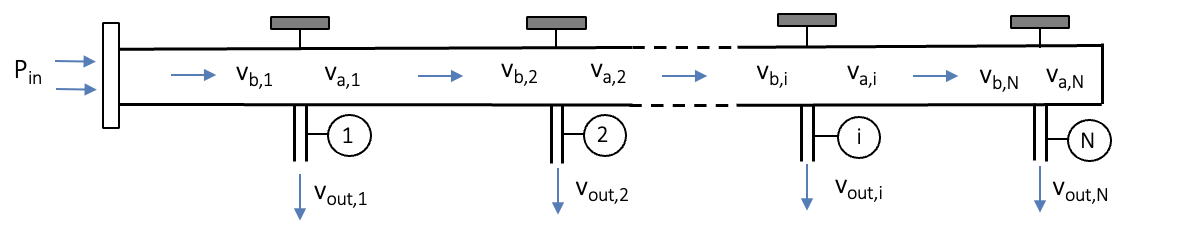
\includegraphics[width=1.\textwidth]{RubinettiInSerie.png}
    \caption{Schematizzazione della serie di rubinetti.}
    \label{fig:figura_1}
\end{figure}
Si consideri una tubazione di diametro $D = 3 cm $ lungo la quale si trovano dei
rubinetti fra loro identici ($d =1 cm$),  posizionati  in serie  a  una  distanza $L = 5
m$ l’uno dall’altro. Questa è alimentata con una portata alla pressione $P_{in} = 1.5
bar$.  Si  considerino  sia  le  perdite di  carico  distribuite lungo  la  tubazione
($\epsilon = 10e^{-5} m$) sia quelle localizzate in prossimità di ciascun rubinetto ($K =
4$). Per il calcolo delle perdite localizzate si utilizzino le velocità appena prima del
corrispettivo rubinetto. Si chiede di:

\begin{enumerate}
    \item Calcolare la velocità d’uscita dal primo rubinetto, supponendo che sia l’unico
       rubinetto presente;
    \item Calcolare il massimo numero di rubinetti in grado di erogare acqua;
    \item Valutare il profilo di pressione assiale lungo la tubazionenelle condizioni del
       punto 2.
\end{enumerate}

Correlazione di Colebrook: 
\begin{equation*}
    \frac{1}{\sqrt{f}} = -4 log_{10} \left(\frac{\frac{\epsilon}{D}}{3.71} +
    \frac{1.256}{Re \sqrt{f}}\right)
\end{equation*}

Il sistema in esame di può schematizzare come riportato in Figura \ref{fig:figura_1}: la
pressione in ingresso $P_{in}$ genera una portata nella tubazione, a stazionario,
proporzionale alla caduta di pressione $P_{in} - P_{atm}$ .

\subsection*{Soluzione}

Se prendiamo in esame il caso in cui solo il primo rubinetto (1) è presente, possiamo
considerare le seguenti 4 incognite del problema:

\begin{enumerate}
    \item $v_{b,1}$: velocità media del fluido prima (il pedice \textbf{b} sta per
       before) del rubinetto 1;
    \item $v_{a,1}$: velocità media del fluido dopo (il pedice \textbf{a} sta per after)
       il rubinetto 1;
    \item $v_{out,1}$: velocità media del fluido in uscita dal rubinetto 1;
    \item $f_{1}$ : il fattore d’attrito (basato sulla velocità $v_{b,1}$ ).
\end{enumerate}

Le 4 equazioni che risolvono il problema sono:

\begin{enumerate}
   \item Equazioni di Bernoulli tra ingresso e uscita dal rubinetto 1:
      \begin{equation*}
         \frac{p_{in}}{\gamma} + \frac{v_{b,1}^{2}}{2g} = \frac{p_{atm}}{\gamma} +
         \frac{v_{out,1}^{2}}{2g} + 4f_{1}\frac{L}{D}\frac{v_{b,1}^{2}}{2g} +
         K_{1}\frac{v_{b,1}^{2}}{2g}
      \end{equation*}

   \item Continuità:
      \begin{equation*}
         v_{b,1}D^{2} = v_{out,1}d^{2} + v_{a,1}D^{2}
      \end{equation*}

   \item Fattore d'attrito:
      \begin{equation*}
         \begin{cases}
            \frac{1}{\sqrt{f_{1}}} =
            \left(-4log_{10}\left(\frac{\epsilon}{3.71D}+\frac{1.256}{\frac{\rho
            v_{b,1}D}{\mu}\sqrt{f_{1}}}\right)\right) \quad per \quad Re_{1} > 2000 \\
            f_{1} = \frac{16 \mu}{\rho v_{b,1}D} \quad per \quad Re_{1} < 2000
         \end{cases}
      \end{equation*}

   \item Condizione di uscita (tubazione con un solo rubinetto, quindi chiusa in fondo):
      \begin{equation*}
         v_{a,1} = 0
      \end{equation*}
\end{enumerate}

Si tratta di un sistema algebrico non lineare, da azzerare numericamente. Si ottiene:

\begin{equation*}
    v_{b,1} = 1.066\frac{m}{s}; \quad v_{a,1} = 0; \quad v_{out,1} = 9.59\frac{m}{s};
    \quad f_{1} = 0.00601
\end{equation*}

Nel caso siano presenti più rubinetti, il procedimento è sostanzialmente analogo: per
ogni rubinetto aggiuntivo andranno scritte quattro nuove equazioni, ottenendo un sistema
algebrico non lineare di $4N$ equazioni, dove $N$ è il numero di rubinetti. Per ogni
rubinetto $i$ si ha quindi:
\begin{enumerate}
   \item Equazioni di Bernoulli tra ingresso e uscita dal rubinetto i (ricordarsi che le
      perdite di carico vanno sommate fino al rubinetto i):
      \begin{equation*}
         \frac{p_{in}}{\gamma} + \frac{v_{b,i}^{2}}{2g} = \frac{p_{atm}}{\gamma} +
         \frac{v_{out,i}^{2}}{2g} + \sum_{j = 1}^{j =
         i}4f_{j}\frac{L}{D}\frac{v_{b,j}^{2}}{2g} + \sum_{j = 1}^{j = i}4f_{j}
         K\frac{v_{b,j}^{2}}{2g}
      \end{equation*}

   \item Continuità:
      \begin{equation*}
         v_{b,i}D^{2} = v_{out,i}d^{2} + v_{a,i}D^{2}
      \end{equation*}

   \item Fattore d'attrito:
      \begin{equation*}
         \begin{cases}
            \frac{1}{\sqrt{f_{i}}} =
            \left(-4log_{10}\left(\frac{\epsilon}{3.71D}+\frac{1.256}{\frac{\rho
            v_{b,i}D}{\mu}\sqrt{f_{i}}}\right)\right) \quad per \quad Re_{i} > 2000 \\
            f_{i} = \frac{16 \mu}{\rho v_{b,i}D} \quad per \quad Re_{i} < 2000
         \end{cases}
      \end{equation*}

   \item Condizione di uscita: si tratta stavolta dell’uguaglianza tra la portata dopo il
      rubinetto $i$ e quella prima del rubinetto $i + 1$, per tutti i rubinetti “interni”
      ($i < N$), mentre la condizione di chiusura per l’ultimo rubinetto ($i = N$):
      \begin{equation*}
         \begin{cases}
            v_{a,i} = v_{b,i+1} \quad per \quad i < N \\
            v_{a,i} = 0 \quad per \quad i = N
         \end{cases}
      \end{equation*}
\end{enumerate}

Per trovare il massimo numero di rubinetti in grado di erogare acqua è necessario
ipotizzare un numero $N$, risolvere il sistema di dimensione $4N\times4N$e verificare che
la portata $v_{out,N}>0$. Analogamente, si può verificare che la pressione dopo il
rubinetto $N$ soddisfi $p_{a,N}>p_{atm}$. È un procedimento dispendioso, ed è necessario
affidarsi ad un risolutore numerico dato l’alto numero di equazioni in gioco.

\end{document}
